\documentclass[dvipdfmx,10pt]{beamer}
\usepackage[utf8]{inputenc}
\usepackage[T1]{fontenc}
\usepackage{lmodern,bm,otf}
\usepackage{graphicx}
\usetheme{default}
\begin{document}
	\author{Hiroki Kato
		Tsuyoshi Goto
		Yong-Rok Kim}
	\title{Charitable Giving, Tax Reform, and Self-selection of Tax Report:
		Evidence from South Korea}
	%\subtitle{}
	%\logo{}
	\institute{Osaka University, Chiba University, Kansai University}
	%\date{}
	%\subject{}
	%\setbeamercovered{transparent}
	%\setbeamertemplate{navigation symbols}{}
	\begin{frame}[plain]
		\maketitle
	\end{frame}
	
	\begin{frame}{Introduction}
		\protect\hypertarget{introduction}{}
		\begin{itemize}
			\item
			In many countries, tax relief for charitable giving are implemented.
			\item
			The elasticity of giving tax relief is known as a key parameter to evaluate the welfare implication (e.g.~Saez, 2004).
			
			\begin{itemize}
				\item
				Intuitively, if the elasticity is more than 1 in absolute value, \$1 of tax relief make more than \$1 of charitable giving.
			\end{itemize}
			\item
			Many papers investigate the elasticity based on tax return data (e.g.~Almunia et al., 2020, Auten et al., 2002, and so on).
		\end{itemize}
	\end{frame}
	
	\begin{frame}{Introduction}
		\protect\hypertarget{introduction-1}{}
		\begin{itemize}
			\item
			However, the tax return data record only the declared charitable giving.
			
			\begin{itemize}
				\item
				First issue: Actual donations is different from declared donations.(Fack and Landais (2016); Gillitzer and Skov (2018))
				\item
				We use panel survey data in South Korea to deal with this issue.
			\end{itemize}
			\item
			Tax payers decide the amount of donation and whether to declare tax relief based on the size of tax incentive and declaration cost.
			
			\begin{itemize}
				\item
				Second issue: Neglect of this declaration cost may bias the estimations of elasticity.
				\item
				We use instrumental variable (IV) and control function approach for this issue.
			\end{itemize}
			\item
			Based on DID as an identification strategy, we investigate the giving price elasticity of South Korea.
		\end{itemize}
	\end{frame}
	
	\begin{frame}{Introduction}
		\protect\hypertarget{introduction-2}{}
		Result
		
		\begin{enumerate}
			\item
			Baseline results show that the giving price elasticity is less than -1.4 in terms of intensive margins and less than -1.7 in terms of extensive margins in Korea.
			\item
			The estimated giving price elasticity for those who declare charitable giving is around -1.2\(\sim\)-1.6.
		\end{enumerate}
		
		These estimates are more elastic than the estimates in the extant research, many of which show around -1.
		
		\begin{enumerate}
			\setcounter{enumi}{2}
			\item
			(Not in the paper) The estimated declaration cost of giving is KRW (\$).
			\item
			(Not in the paper) Given our estimates, increasing the subsidy on charitable giving will be desirable in Korea.
		\end{enumerate}
	\end{frame}
	
	\begin{frame}{2014 tax reform in South Korea}
		\protect\hypertarget{tax-reform-in-south-korea}{}
		In Korea, income tax payers can receive tax relief for their charitable giving.
		
		\begin{itemize}
			\item
			For the application of tax relief, tax payers have to submit a certificate for charitable giving.
			\item
			Wage earners pay their income tax by withholding tax and declare their charitable giving via their company.
			
			\begin{itemize}
				\item
				Wage earners can submit the certificate at any time.
			\end{itemize}
			\item
			Non wage earners, such as the self-employed, pay their income tax by tax-return and declare their charitable giving via the National Tax Service.
			
			\begin{itemize}
				\item
				Non wage earners have to retain the certificate until they submit tax return.
			\end{itemize}
		\end{itemize}
	\end{frame}
	
	\begin{frame}{2014 tax reform in South Korea}
		\protect\hypertarget{tax-reform-in-south-korea-1}{}
		Our major price variation comes from the 2014 tax reform.
		
		\begin{itemize}
			\item
			Before 2014, tax deduction (所得控除) was used for tax relief on charitable giving.
			
			\begin{itemize}
				\item
				I.e. the giving price depended on income level.
			\end{itemize}
			\item
			After 2014, tax credit (税額控除) started to be used for tax relief on charitable giving.
			
			\begin{itemize}
				\item
				The tax credit rate was determined as 15\%.
				\item
				Giving price is 0.85, irrespective of income level.
			\end{itemize}
		\end{itemize}
	\end{frame}
	
	\begin{frame}{2014 tax reform in South Korea}
		\protect\hypertarget{tax-reform-in-south-korea-2}{}
		Model
		
		\begin{itemize}
			\item
			Consider private consumption (\(x_{i}\)) and charitable giving (\(g_{i}\)).
			\item
			The budget constraint is
		\end{itemize}
		
		\[x_{i} + g_{i} = y_{i} - R_iK- R_iT(y_{i}, g_{i})-(1-R_i)T(y_i)\]
		
		where \(y_{i}\) is pre-tax total income, \(R_{i}\) is a dummy of declaration of tax relief and \(T(y_i)\) and \(T(y_{i}, g_{i})\) are respectively the amount of tax when \(i\) does not declare tax relief and when \(i\) declares tax relief.
		
		\begin{itemize}
			\item Tax payers declare their charitable giving if its benefit exceeds its cost.
			\begin{align}
				R_i=\begin{cases}
					1 \text{ if }T(y_i, g_i) - T(y_i)>K\\
					0 \text{ if }T(y_i, g_i) - T(y_i)\le K.
				\end{cases}
			\end{align}
		\end{itemize}
	\end{frame}
	
	\begin{frame}{2014 tax reform in South Korea}
		\textbf{Tax deduction system (until 2013)}
		\[T(y_{i}, g_{i}) = T(y_{i} - g_{i})\]
		
		\begin{itemize}
			\item In 2012 and 2013, the marginal tax rate was the same, though it was different from ones before 2011.
			\item The logged relative giving price is \(R_{i}\ln(1 - T'(y_{i} - g_{i}))\).
		\end{itemize}
		
		\textbf{Tax credit system (from 2014)}
		\[T(y_{i}, g_{i}) = T(y_{i}) - R_{i} m g_{i}\]
		
		\begin{itemize}
			\item \(m\) is tax credit rate and is \(m = 0.15\).
			\item The logged relative giving price is \(R_{i}\ln(1 - 0.15) = R_{i}\ln 0.85\).
		\end{itemize}
		
		Note: The logged relative giving price for the non-declared is \(\ln1 =0\).
	\end{frame}
	
	\begin{frame}{Source of endogeneity}
		\begin{enumerate}
			\item Usage of tax return data only captures declared charitable giving.
			\begin{itemize}
				\item If the charitable giving is not declared, tax relief has a little effect.
				\item Some papers use survey data to deal with this problem (e.g.~Rehavi and Shack, 2013).
				\item \textbf{Following them, we use survey panel data of Korea.}
			\end{itemize}
			\item If the declaration cost is ignored, the estimation should be biased.
			\begin{itemize}
				\item The giving price depends not only on marginal tax rate and tax credit rate, but also on the declaration behavior.
				\item As far as we know, only Almunia et al.~(2020) deal with this problem, though they used tax return data.
				\item\textbf{We use the different declaration cost btw wage earners and the others as an instrumental variable (IV).}
			\end{itemize}
		\end{enumerate}
	\end{frame}
	
	\begin{frame}{Data}
		We use the Korean annual financial panel survey, called the National Survey of Tax and Benefit (hereafter, NaSTab).
		\begin{itemize}
			\item The subjects of this survey are general households and household members living in 15 cities and provinces nationwide.
			\item This survey is based on a face-to-face interview.
			\item Data is constructed as the subjects represent the population of Korean society.
			\item We exclude the subject of the sample, whose age is under 23, since they are not likely to have income or assets.
			\item We use data from 2013 to 2017.
		\end{itemize}
	\end{frame}

\begin{frame}{Data}
	\begin{figure}
		\centering
		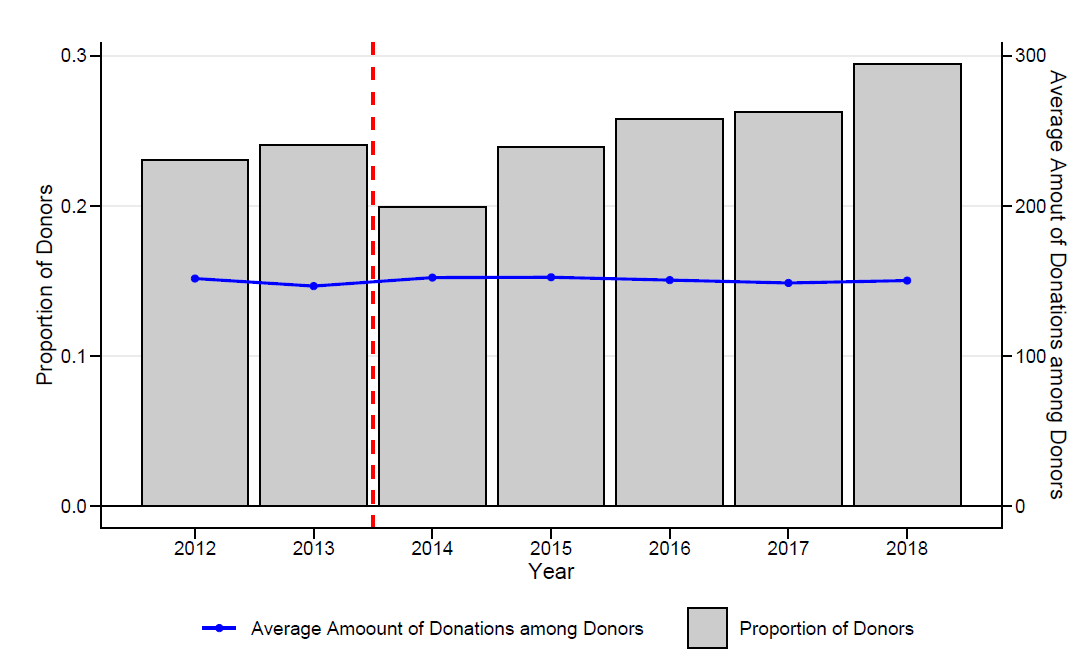
\includegraphics[width=0.8\linewidth]{Fig_Average_donation}
		\caption{Proportion of Donors and Average Donations among Donors}
		\label{fig:1}
	\end{figure}
\small
	\begin{itemize}
		\item About 20$\sim$30\% of people make a donation.
		\item The average amount of donations among donors is about 1.5 million KRW.
	\end{itemize}
\end{frame}

\begin{frame}{Data}
	\begin{figure}
		\centering
		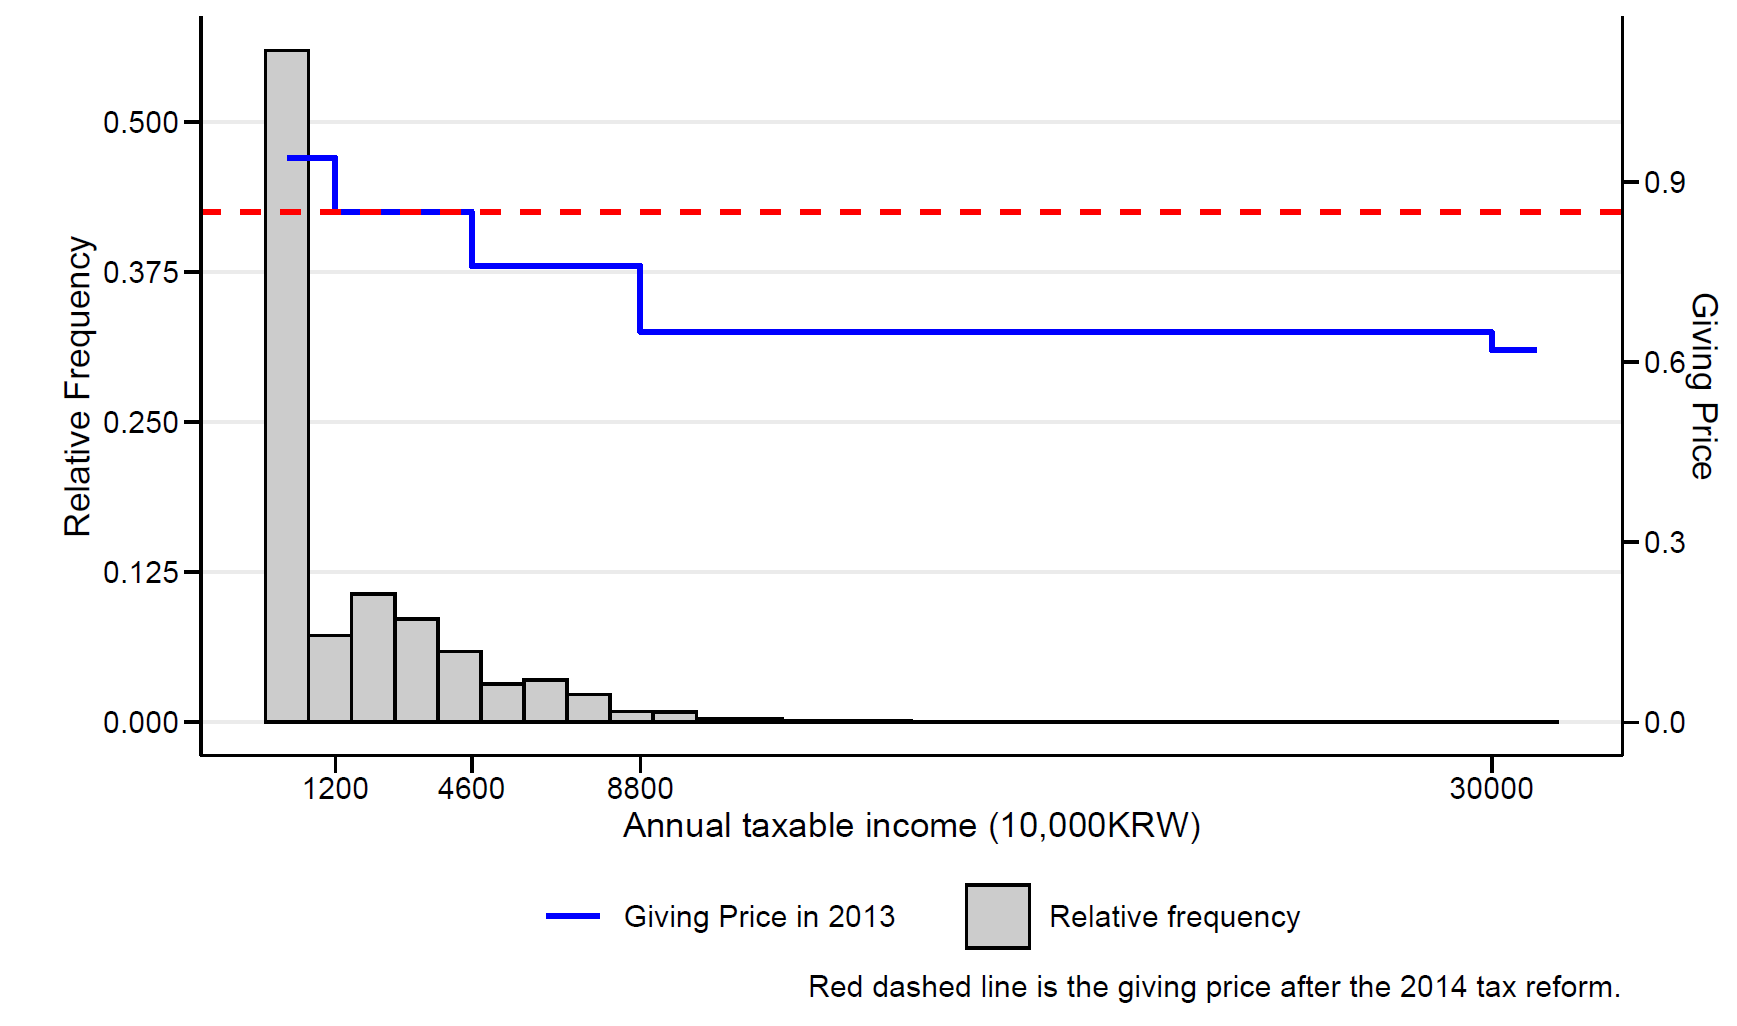
\includegraphics[width=0.7\linewidth]{Fig_Income_distribution}
		\caption{Income Distribution and Relative Giving Price in 2013}
		\label{fig:2}
	\end{figure}
\small
	In 2014, relative giving price
	\begin{itemize}
		\item decreases for people whose income is less than 12 million KRW.
		\item is the same for people whose income is between 12 million KRW and 46 million KRW.
		\item increase for people whose income is more than 46 million KRW.
	\end{itemize}
\end{frame}

\begin{frame}{Data}
	\begin{figure}
		\centering
		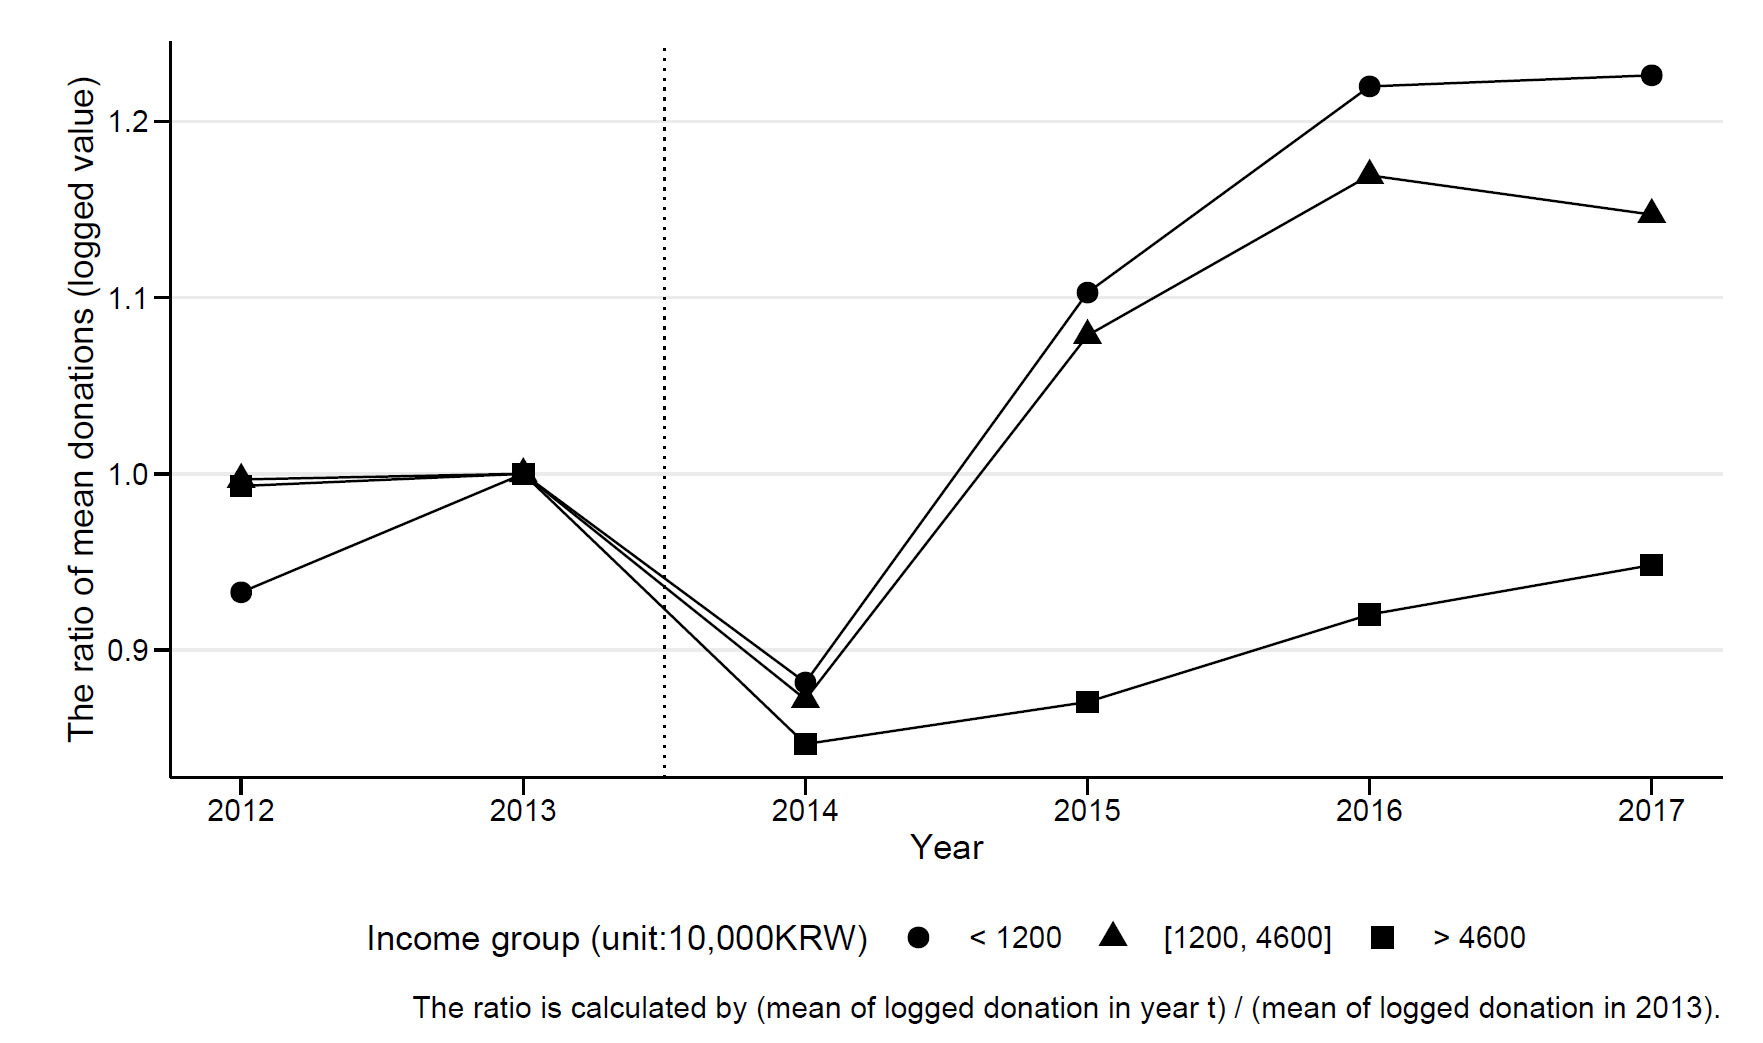
\includegraphics[width=0.7\linewidth]{Fig_Diff}
		\caption{Average Logged Giving in Three Income Groups}
		\label{fig:3}
	\end{figure}
\small
	Compared to 2012 and 2013, the amount of charitable giving after 2014
	\begin{itemize}
		\item increases for people whose income is less than 12 million KRW.
		\item relatively increases for people whose income is between 12 million KRW and 46 million KRW.
		\item decreases for people whose income is more than 46 million KRW.
	\end{itemize}
\end{frame}

\begin{frame}{Data}
	\begin{figure}
		\centering
		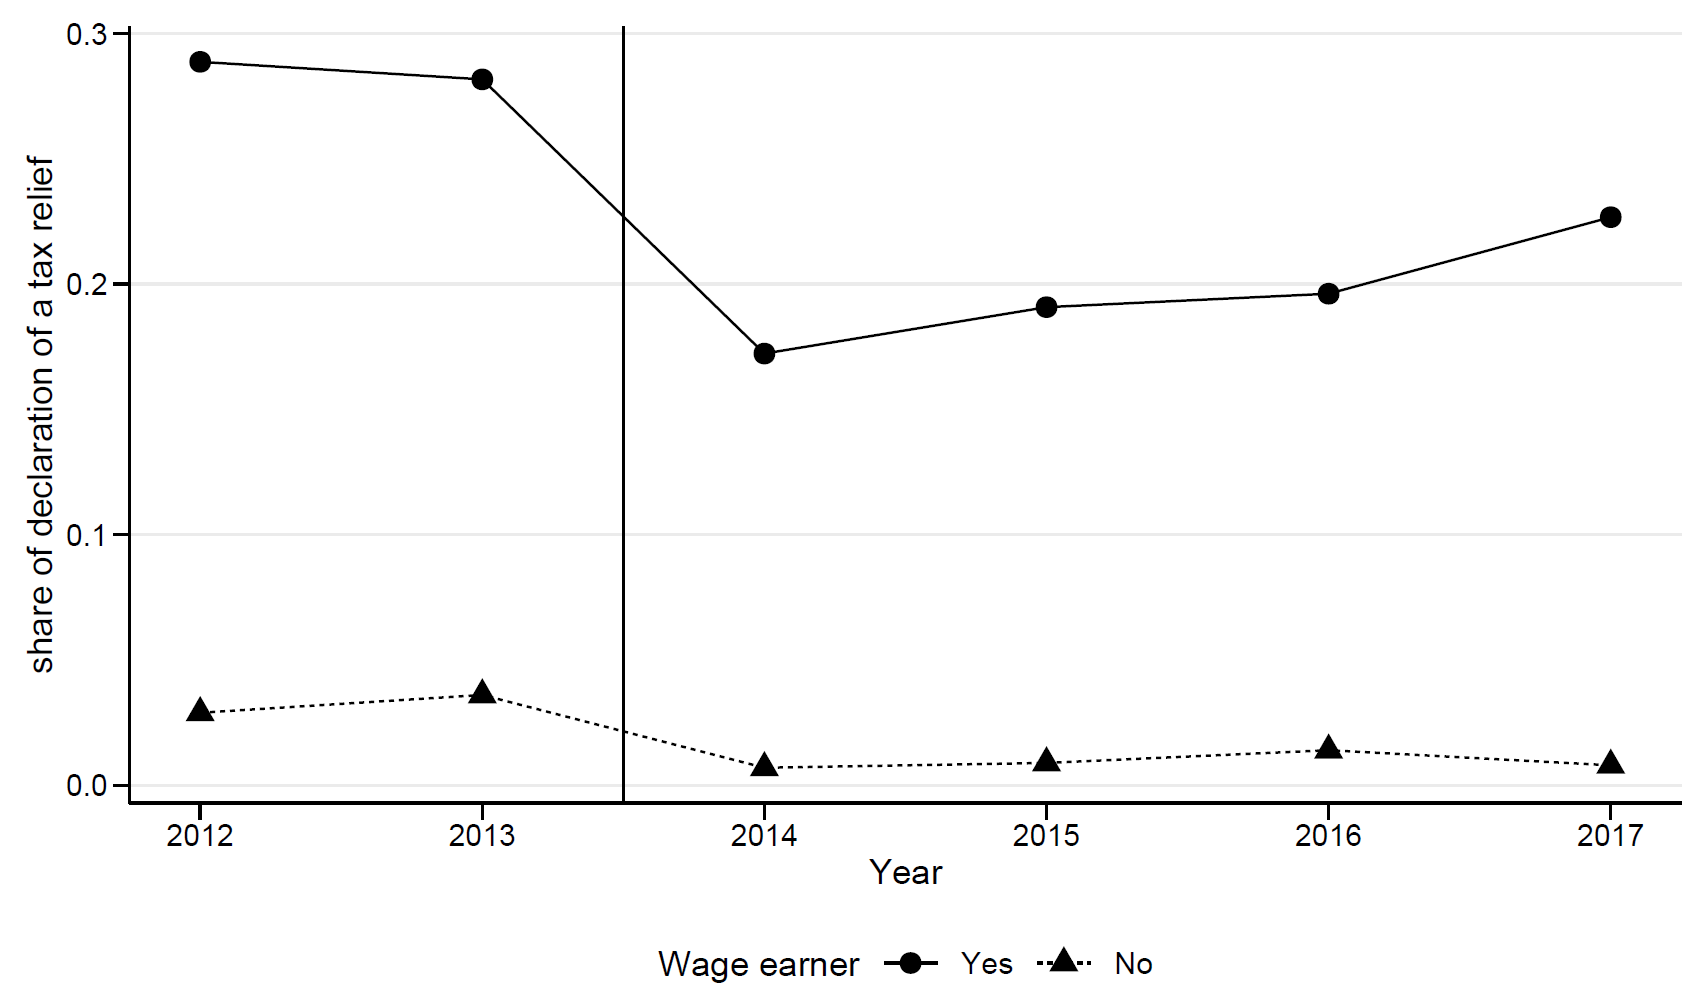
\includegraphics[width=0.7\linewidth]{Fig_Declaration}
		\caption{Share of Declaration of Tax Relief}
		\label{fig:4}
	\end{figure}
\small
	\begin{itemize}
		\item Wage earners are more likely to declare their charitable giving to receive tax relief.\\
		$\to$ This reflects the difference of the declaration cost.
	\end{itemize}
\end{frame}

\begin{frame}{Data}
	\begin{table}
		\centering
		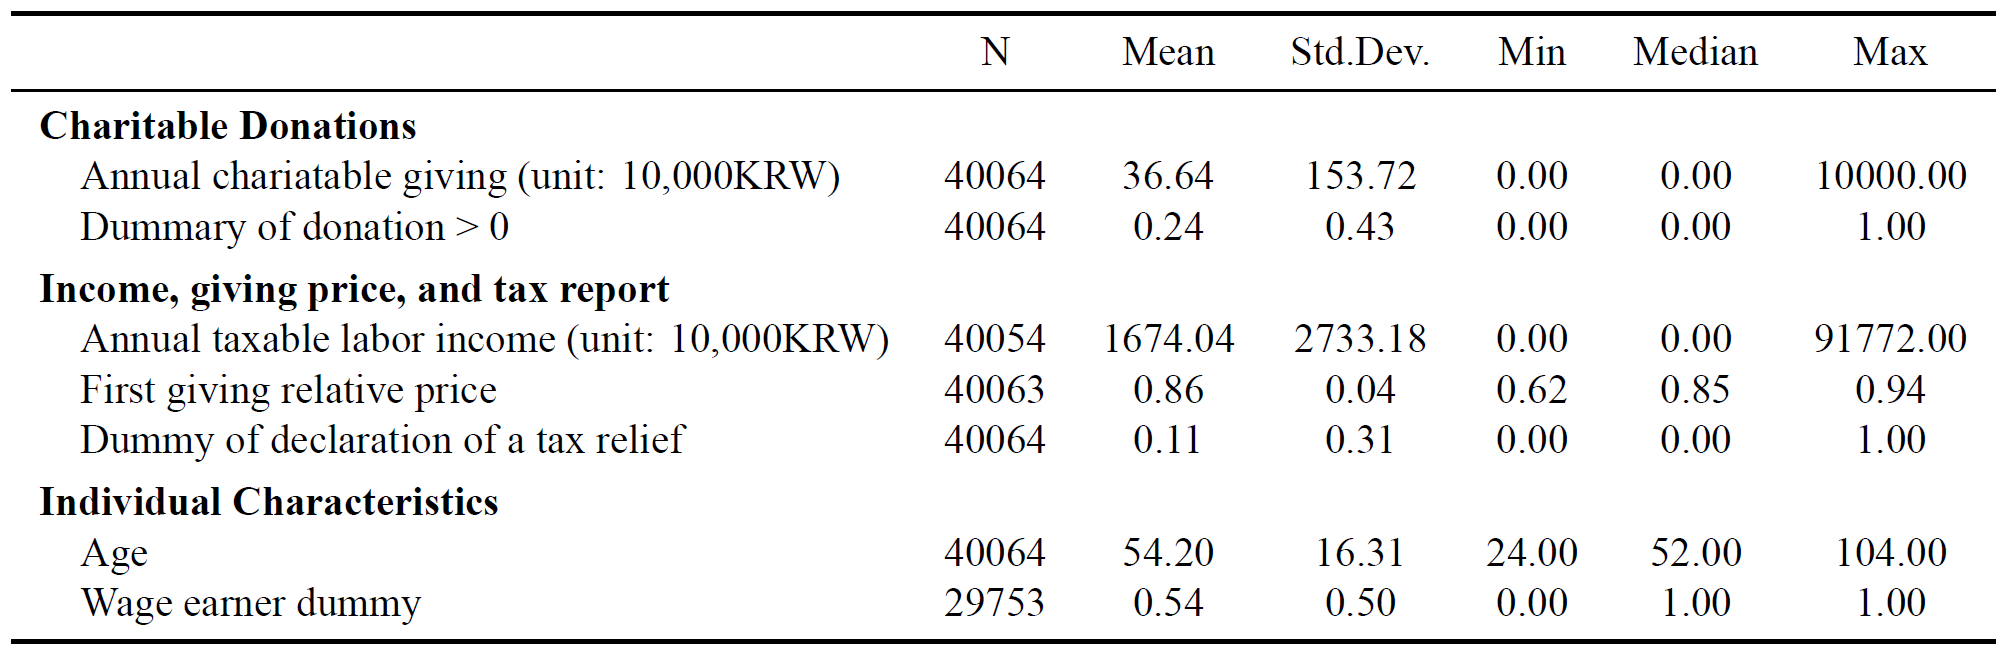
\includegraphics[width=0.9\linewidth]{Tab_Stat}
		\caption{Summary Statistics}
		\label{tab:1}
	\end{table}
\end{frame}

\begin{frame}{Statistical Model}
\begin{itemize}
	\item Main identification source is tax reform in 2014. (DID-like strategy)
	\begin{itemize}
		\item Below 12 million KRW: Giving price decreases.
		\item Btw 12 and 46 million KRW: Giving price is the same.
		\item Above 46 million KRW: Giving price increases.
	\end{itemize}
	\item To capture the difference of declaration cost, we use a dummy to show whether a subject is a wage earner or not as IV.
\end{itemize}
\end{frame}

\begin{frame}{Statistical Model}
	\begin{itemize}
		\item We estimate the following two-way fixed effect model:
		\begin{align}
			\ln g_{it} = \varepsilon_pR_{it} \ln p_{it}(y_{it}, g_{it}) + \varepsilon_y \ln y_{it} + \bm{X}_{it}\bm{\beta} + \mu_i + \iota_t + u_{it}\tag{5}
		\end{align}
	where $\mu_i, \iota_t$ and $ u_{it}$ are an individual fixed effect, a year fixed effect, and a error term, respectively. 
	\item $\bm{X}_{it}$ is a vector of covariates including square of age, industry dummy, and area dummy.
	\item In the literature, estimations in terms of \textbf{intensive} and \textbf{extensive} margins are common.
	\begin{itemize}
		\item \textbf{Intensive margins}: estimate (5) only for $g_{it}>0$.
		\item \textbf{Extensive margins}: estimate (5) but dependent variable is $1[g_{it}>0]$.
	\end{itemize}
	$\to$ Following the literature, we estimate both of them.
	\end{itemize}
\end{frame}

\begin{frame}{Statistical Model: Endogeneity of $p_{it}$}
	\begin{itemize}
		\item The giving price (compared to private good) is
		\begin{align}
			p_{it}(y_{it}, g_{it})=\begin{cases}
			1-T'_t(y_{it}-g_{it})&\text{ if }t<2014\\
			0.85&\text{ if }t\ge2014
			\end{cases}
			\tag{6'}.
		\end{align}
		\item Since the giving price is endogenous to the amount of giving before 2014, we use ``\textbf{the first-price of giving}", which is defined as 
		\begin{align}
			p_{it}^f(y_{it})=p_{it}(y_{it},0)\notag
		\end{align}
		 instead of $p_{it}(y_{it},0)$ in the estimation.
		\item $p_{it}(y_{it},0)$ is called as ``the last-price of giving".
	\end{itemize}
\end{frame}

\begin{frame}{Statistical Model: Endogeneity of $R_{it}$}
	\begin{itemize}
		\item Since donors can choose whether they declare charitable giving or not, declaration, $R_{it}$, is endogenous.
		\item To overcome this, we estimate 
		\begin{align}
			\ln g_{it} = \varepsilon_pR_{it} \ln p_{it}^f(y_{it}) + \varepsilon_y \ln y_{it} + \bm{X}_{it}\bm{\beta} + \mu_i + \iota_t + u_{it}\tag{7}
		\end{align}
	 	where $R_{it} \ln p_{it}^f(y_{it})$ is instrumented by $WageEarner_{it}\times \ln p^f_{it}(y_{it})$. 
	 	\begin{itemize}
	 		\item This estimation is based on 2SLS.
	 	\end{itemize}
		\item $WageEarner_{it}$ is a dummy to show whether a subject is a wage earner or not.
		\begin{itemize}
			\item $WageEarner_{it}$ should not correlate to $u_{it}$ when we control incomes and industry dummies.
		\end{itemize}
	\end{itemize}
\end{frame}

\begin{frame}{Statistical Model: Endogeneity of $R_{it}$}
	\begin{itemize}
		\item In alternative models, we use propensity score to declare $P(Z_{it})$ as an instrument.
		\begin{itemize}
			\item This estimation method is called ``control function (CF)" approach.
			\item The propensity score is estimated by a probit model
			\begin{align}
				R_{it}=1[\delta_0+Z_{it}\delta_1+u_{it1}>0]\tag{8},
			\end{align}
			where $Z_{it}\equiv \{WageEarner_{it}, \ln p_{it}^f(y_{it}), \ln y_{it}, \bm{X}_{it}\}$.
			\item The propensity score is $P(Z_{it})=\Phi(\hat{\delta}_0+Z_{it}\hat{\delta}_1)$.
			\item We consider two cases:\\
			 \ajMaru1 pooled probit model $(\delta_0, \delta_1)$ is constant.\\
			 \ajMaru2 separated probit model $(\delta_0, \delta_1)$ can vary by year.
		\end{itemize}
		\item In addition, we also estimate the following by OLS:
		\begin{align}
			\ln g_{it} = \varepsilon_pP(Z_{it})\ln p_{it}^f(y_{it}) + \varepsilon_y \ln y_{it} + \bm{X}_{it}\bm{\beta} + \mu_i + \iota_t + u_{it}\tag{9}
		\end{align}
	\end{itemize}
\end{frame}

\begin{frame}{Results: Intensive Margins}
	\begin{table}
		\centering
		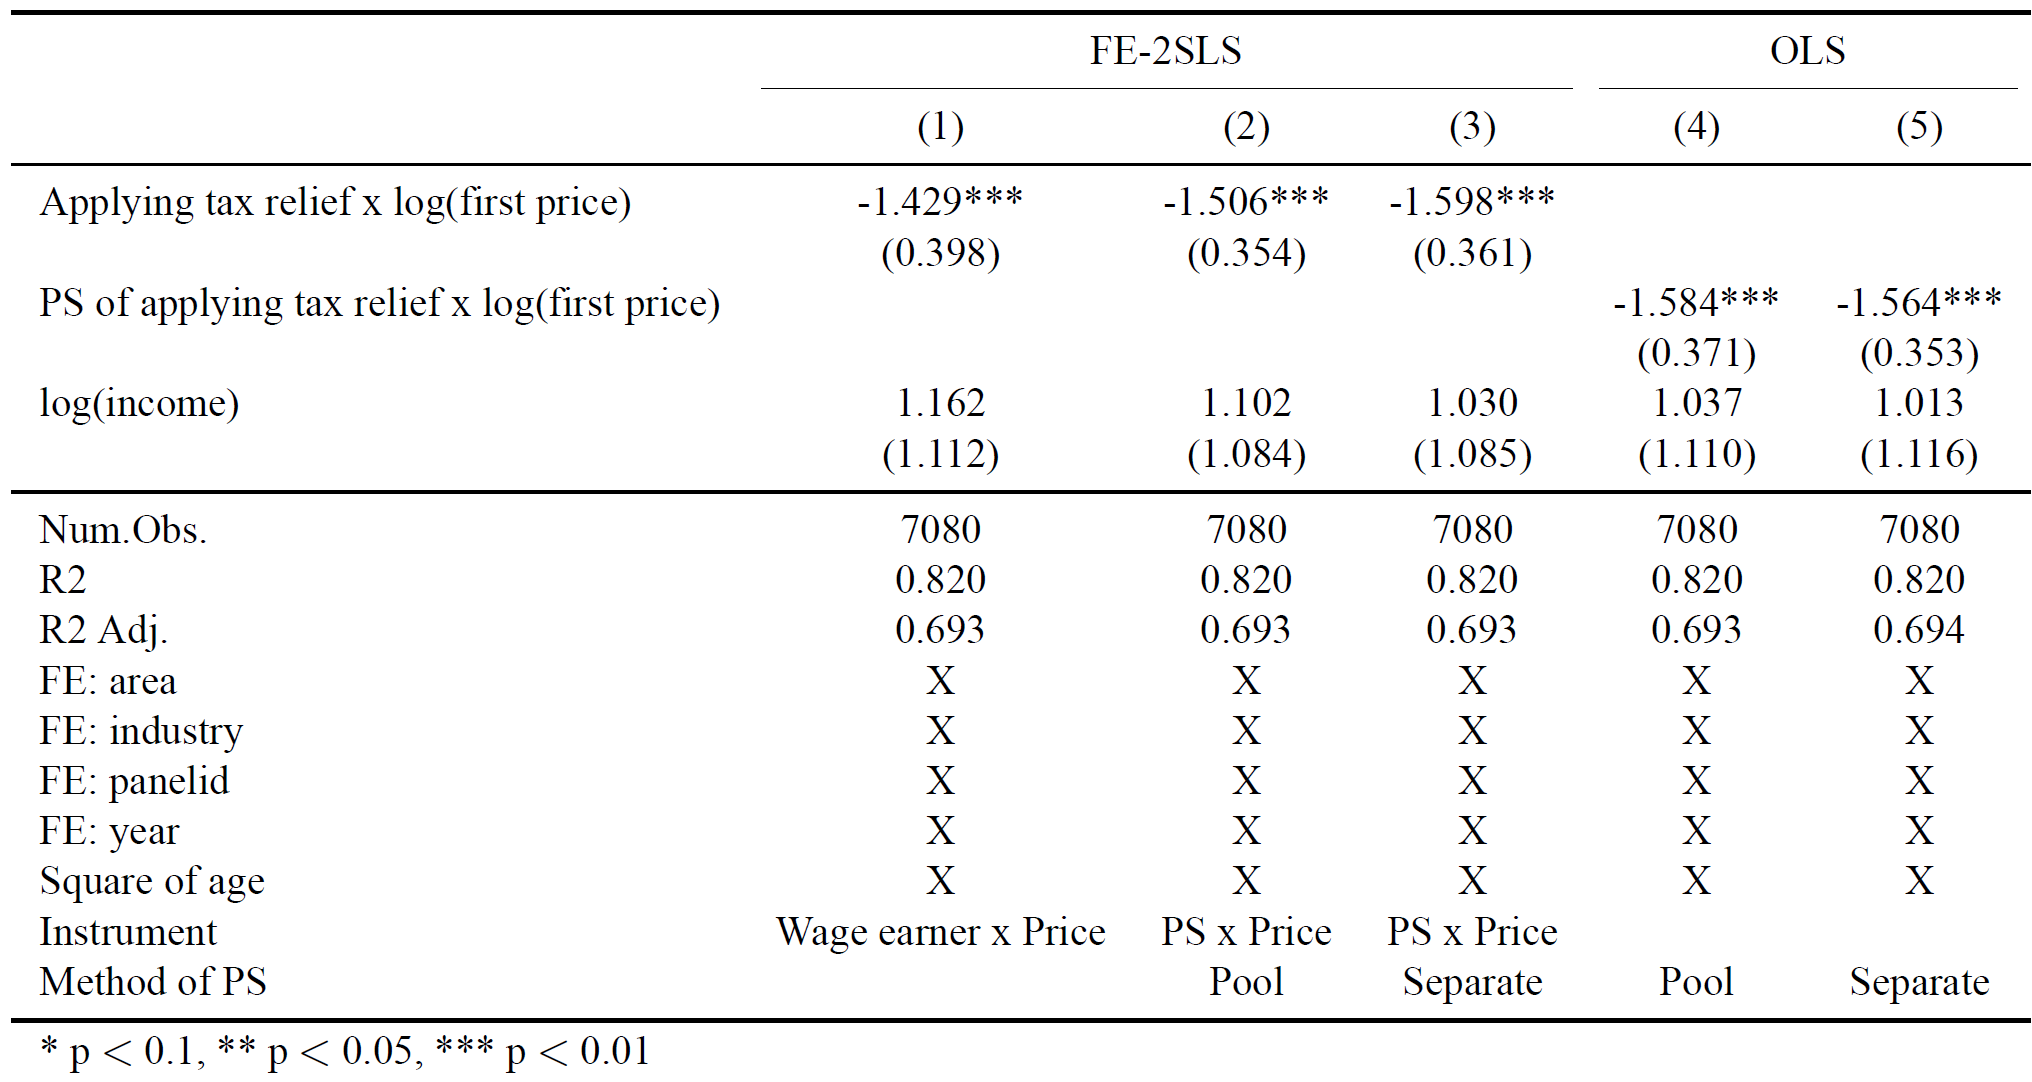
\includegraphics[width=0.9\linewidth]{Tab_res_1}
		\caption{First-Price Elasticities (Intensive Margins)}
		\label{tab:2}
	\end{table}
The estimated giving price elasticity in terms of intensive margins is about -1.5.
\end{frame}

\begin{frame}{Results: Extensive Margins}
	\begin{table}
		\centering
		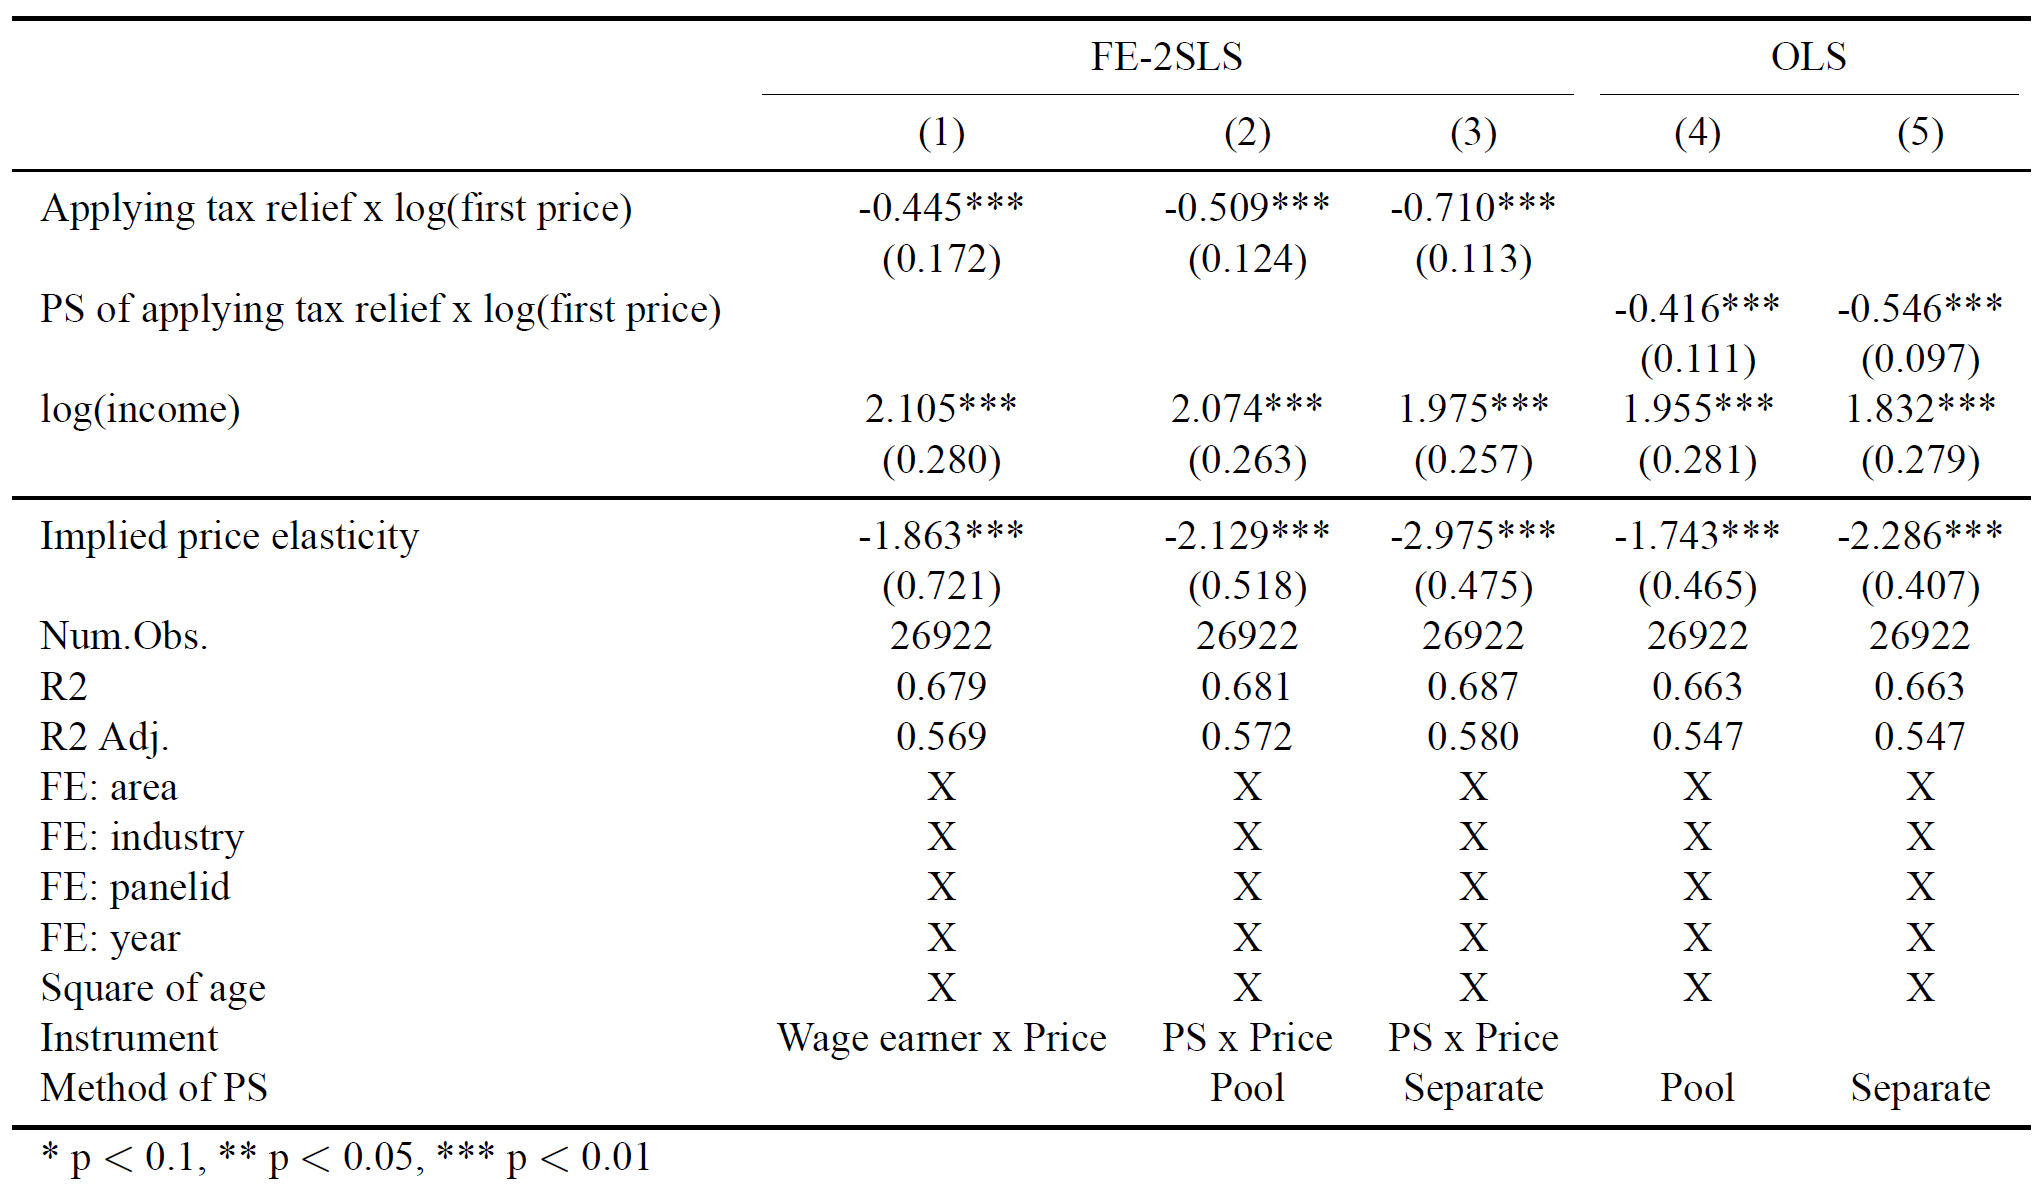
\includegraphics[width=0.9\linewidth]{Tab_res_2}
		\caption{First-Price Elasticities (Extensive Margins)}
		\label{tab:3}
	\end{table}
	The estimated giving price elasticity in terms of extensive margins is about -1.7 $\sim$ -2.9.
\end{frame}

\begin{frame}{Results}
	\begin{itemize}
		\item The results show that the giving price elasticity in Korea is more elastic than many papers in the literature show.
		\begin{itemize}
			\item In the literature, the giving price elasticity in terms of intensive margins is typically -1.
		\end{itemize}
		\item The elasticity in terms of extensive margins captures the behavior of whether people donate or not.
		  \begin{itemize}
		  	\item The elastic extensive margins elasticity shows that reducing giving price induce people to donate.
		  	\item IVを使わない場合の推定結果が得られるならば、ここでIVを使わない推定結果と比べたときの含意を書く。
		  \end{itemize}
	\end{itemize}
\end{frame}

\begin{frame}{Results}
 We try several robustness checks.
		\begin{enumerate}
			\item Estimation excluding 2013 and 2014 data: to eliminate announcement effect.
			\item Estimation using the last-price
			\item Estimation using the subsample of those who have applied for tax relief
			\begin{itemize}
				\item We use Semykina and Wooldridge (2010)'s way of the correction of sample selection bias.
				\item Estimated elasticity (intensive margins) is around -1.2\(\sim\)-1.6.
				\item Subsample analysis enables us to use several methods to deal with issues related to tax deduction system.\\
				e.g. fluctuation of income level (Randolph, 1995, and so on.)\\
				$\to$ usage of k-th difference model / lead and lag.  
			\end{itemize}
		\end{enumerate}
		Most of result shows that the giving price elasticity is less than
		\begin{itemize}
			\item -1.4 in terms of intensive margins and 
			\item -1.7 in terms of extensive margins.
		\end{itemize}
\end{frame}

\begin{frame}{Implications for the welfare (not in the paper)}
	Following Almunia et al. (2020), we can derive the welfare implication by specifying the following utility maximization.
	\begin{align}
		\max_{x_i,g_i,R_i}&U(x_i,g_i,G)= x_i - R_iK +\theta u(g_i) + V(G)\notag\\
		\text{s.t. }&x_i + g_i = R_i(y-T(y, g_i)) + (1-R_i)(y-T(y)),\notag\\
		&\text{ and }G=g_i+G_{-i}\notag,
	\end{align}
	where $\theta\in[\underline{\theta},\bar{\theta}$] is the parameter to show the preference for donation, which follows the density $f(\cdot)$. 
	\begin{itemize}
		\item $G$ is the total donation (including the governmental provision).
		\item $G_{-i}$ is the total donation except $i$.
		\item For simplicity, assume tax schedule is now linear and tax rate is $\tau$.
	\end{itemize}
\end{frame}

\begin{frame}{Implications for the welfare (not in the paper)}
	\begin{itemize}
	\item Then, the optimization will be
	\begin{align}
		\max_{g_i,R_i} (1-\tau)y-R_ipg_i-(1-R_i)g_i- R_iK +\theta u(g_i)+V(G).\notag
	\end{align}
	\item Denote $g(p;\theta)$ and $g(1; \theta)$ as the donation when $R_i=1$ and $0$.
	\item As a result of the optimization, the indirect utility of those who declare giving and do not will respectively be
	\begin{align}
		\nu(p;\theta)&=\theta_i u(g(p;\theta))-pg(p;\theta)\notag\\
		\nu(1;\theta)&=\theta_i u(g(1;\theta))-g(1;\theta)\notag.
	\end{align}
\end{itemize}
\end{frame}

\begin{frame}{Implications for the welfare (not in the paper)}
	\begin{itemize}
		\item Depends on $\theta$ and giving price $p$, three types of individuals exist.
		\begin{enumerate}
			\item Non-donor: $\theta\le \theta_0$
			\item Donor but non-declarer: $\theta\in(\theta_0,\theta(p)]$\\
			$\to$ Denote their total donation as $g^0(p)\equiv\int_{\theta_0}^{\theta(p)}g(1;\theta)f(\theta)d\theta$.
			\item Donor and declarer: $\theta>\theta(p)$\\
			$\to$ Denote their total donation as $g^1(p)\equiv\int_{\theta(q)}^{\bar{\theta}}g(p;\theta)f(\theta)d\theta$.
		\end{enumerate}
	\item Social welfare can be written as
	\begin{align}
		W=V(G)&+\int_{\theta(p)}^{\bar{\theta}}(\nu(p;\theta)-K)f(\theta)d\theta\notag\\
		&+\int_{\theta_0}^{\theta(p)}\nu(1;\theta)f(\theta)d\theta+\lambda[ty-(1-p)g^1(p)-G_g]\notag
	\end{align}
	where $\lambda$ is the marginal cost of public finance.
	\end{itemize}
\end{frame}

\begin{frame}{Implications for the welfare (not in the paper)}
	\begin{itemize}
		\item Using $\lambda=V'$ (Saez, 2004), the effect of changing giving price $p$ on the welfare $W$ can be shown as 
		\begin{align}
			\frac{dW}{dp} =\lambda (g_p^0+g_p^1)+(\lambda-1)g^1-\lambda(1-p)g_p^1\notag.
		\end{align}
		\item $\frac{dW}{dp}<0$ is equivalent to
		\begin{align}
			\epsilon\equiv -\frac{pg_p^1}{g^1}>\frac{\lambda-1}{\lambda}+\frac{g_p^0}{g^1}\notag.
		\end{align}
		\begin{itemize}
		\item From the subsample analysis, $\epsilon$ is 1.304 $\sim$ 1.603.
		\item Assuming $\lambda\in[1,2]$, $\frac{\lambda-1}{\lambda}\in[0,\frac12]$.
		\item From the data, $\frac{g_p^0}{g^1}$ is 0.00003.
		\end{itemize}
		\item Our result suggests that more generous tax relief will increase the welfare in Korea.
	\end{itemize}
\end{frame}
\end{document}